\begin{figure}[!htb]
\centering
\begin{subfigure}[t]{0.48\linewidth}
  \centering
  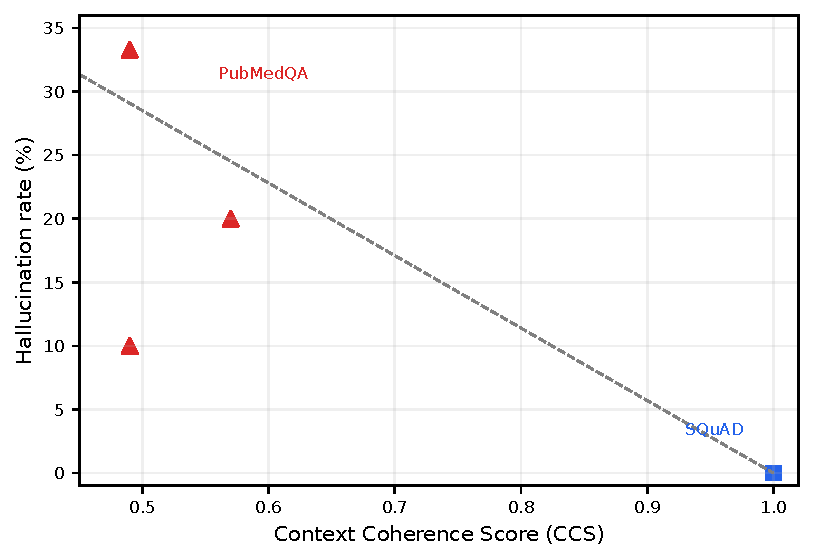
\includegraphics[width=\linewidth]{ccs_hallucination.pdf}
  \caption{CCS vs.\ hallucination. Low-coherence retrieval sets coincide with higher hallucination at the aggregate level.}
  \label{fig:ccs_hallucination}
\end{subfigure}
\hfill
\begin{subfigure}[t]{0.48\linewidth}
  \centering
  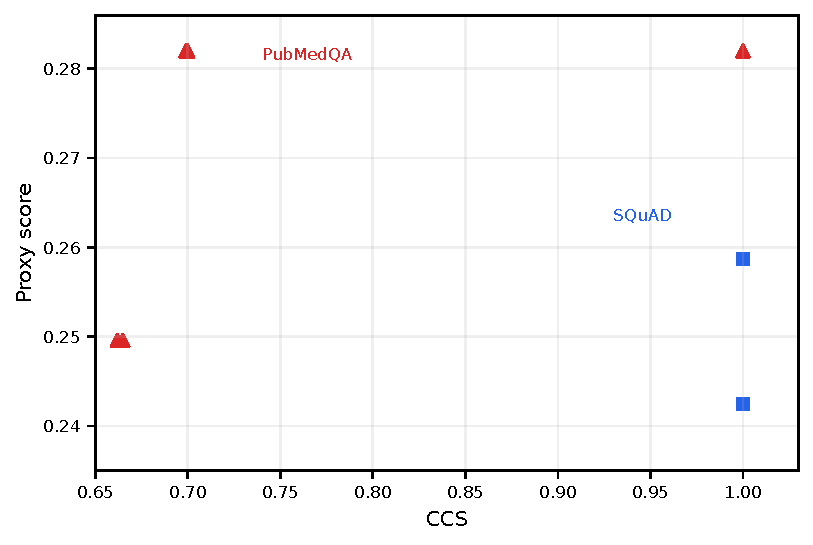
\includegraphics[width=\linewidth]{proxy_alignment.pdf}
  \caption{Proxy-based tuning aligns with CCS, identifying the same high-performing regions without requiring generation.}
  \label{fig:proxy}
\end{subfigure}
\caption{CCS as a retrieval-time diagnostic. (a)~Although CCS is not a per-query oracle, the aggregate trend is monotonic: conditions with CCS = 1.0 show 0\% hallucination, while CCS = 0.57 coincides with 20\%. (b)~A proxy score combining CCS, embedding variance, retrieval entropy, and mean query-chunk similarity tracks the same operating regions as full answer-level evaluation, enabling inexpensive threshold search.}
\label{fig:ccs_proxy_combined}
\end{figure}
